\begin{grafica}[H]
\centering
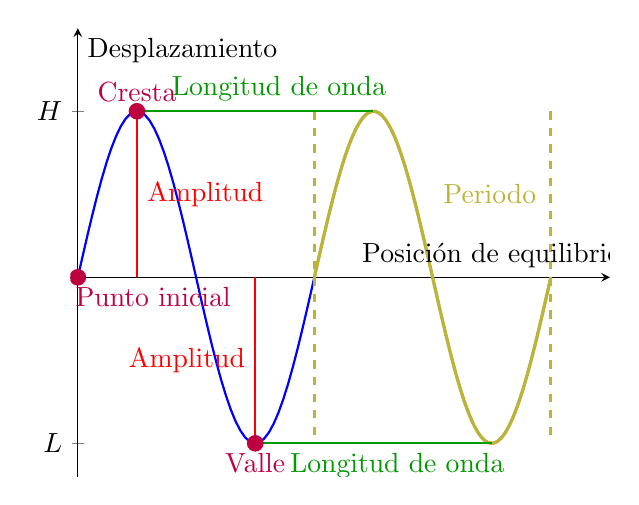
\begin{tikzpicture}
  \begin{axis}[
    xmin=-0.2,xmax=4.5*pi,
    ymin=-1.2,ymax=1.5,
    axis lines=middle,
    xtick={0},
    % xtick={pi/2,pi,3*pi/2,2*pi,5*pi/2,3*pi,7*pi/2,4*pi},
    % xticklabels={
    %   $\dfrac{\pi}{2}$,
    %   $\pi$,
    %   $\dfrac{3}{2}\pi$,
    %   $2\pi$,
    %   $\dfrac{5}{2}\pi$,
    %   $3\pi$,
    %   $\dfrac{7}{2}\pi$,
    %   $4\pi$
    % },
    ytick={-1,1},yticklabels={$L$,$H$},
    ylabel=Desplazamiento
    ]

    % Funcion senoidal
    \addplot[color=blue,samples=100,domain=0:4*pi,thick]{sin(deg(x))};

    % Punto inicial
    \fill[purple] (axis cs:0,0) circle[radius=3pt];
    \node[purple,below] at (axis cs:2,0) {Punto inicial};

    % Periodo
    \addplot[color=yellow!70!black,samples=100,domain=2*pi:4*pi,very thick]{sin(deg(x))};
    \node[yellow!70!black,right,very thick] at (axis cs:3*pi,0.5) {Periodo};
    \draw[yellow!70!black,dashed,very thick] (axis cs:2*pi,1) -- (axis cs:2*pi,-1);
    \draw[yellow!70!black,dashed,very thick] (axis cs:4*pi,1) -- (axis cs:4*pi,-1);

    % Amplitud
    \draw[red,thick] (axis cs:pi/2,0) -- (axis cs:pi/2,1) node[pos=0.5,right] {Amplitud};
    \draw[red,thick] (axis cs:3*pi/2,0) -- (axis cs:3*pi/2,-1) node[pos=0.5,left] {Amplitud};

    % Longitud de onda
    \draw[green!60!black,thick] (axis cs:pi/2,1) -- (axis cs:5*pi/2,1) node[pos=0.6,above] {Longitud de onda};
    \draw[green!60!black,thick] (axis cs:3*pi/2,-1) -- (axis cs:7*pi/2,-1) node[pos=0.6,below] {Longitud de onda};

    % Cresta
    \fill[purple] (axis cs:pi/2,1) circle[radius=3pt];
    \node[purple,above] at (axis cs:pi/2,1) {Cresta};

    % Valle
    \fill[purple] (axis cs:3*pi/2,-1) circle[radius=3pt];
    \node[purple,below] at (axis cs:3*pi/2,-1) {Valle};

    % Posicion de equilibrio
    \node[above] at (axis cs:7*pi/2,0) {Posición de equilibrio};
  \end{axis}
\end{tikzpicture}
\caption{Elementos de una onda}
\end{grafica}
